\documentclass[11pt]{article}

\usepackage[a4paper, margin=0.9in]{geometry}
\usepackage[T1]{fontenc}
\usepackage[utf8]{inputenc}
\usepackage[charter]{mathdesign}
\usepackage{microtype}
\usepackage{booktabs}
\usepackage{longtable}
\usepackage{array}
\usepackage{xcolor}
\usepackage{tikz}
\usetikzlibrary{positioning, arrows.meta, patterns}
\usepackage{pgfplots}
\pgfplotsset{compat=1.18}
\usepackage{caption}
\usepackage{float}
\usepackage{enumitem}
\usepackage[hidelinks]{hyperref}

% ── palette ──────────────────────────────────────────────────
\definecolor{hexblue}{HTML}{2A78D6}
\definecolor{hexorange}{HTML}{EB6834}
\definecolor{hexaqua}{HTML}{1BAF7A}
\definecolor{hexgray}{HTML}{898781}
\definecolor{inkmuted}{HTML}{52514E}
\definecolor{rulegray}{HTML}{E1E0D9}
\definecolor{hexred}{HTML}{D03B3B}

\captionsetup{font=small, labelfont={bf}, width=0.92\textwidth, skip=4pt}
\setlist{itemsep=1pt, topsep=3pt}
\setlength{\textfloatsep}{10pt}
\setlength{\intextsep}{8pt}

\newcommand{\code}[1]{\texttt{\small #1}}

\title{\textbf{Hex CLI: A Measurement-First Coding Agent\\ on a 4-Billion-Parameter Model and a Laptop NPU}}
\author{Nathan L.\\ \small\texttt{github.com/NathanL15/Hex-CLI}}
\date{September 2026 \,\textperiodcentered\, v2.8.0}

\begin{document}
\maketitle

\begin{abstract}
\noindent
Hex CLI is a terminal coding agent in the tradition of Claude Code, with one
structural difference: it runs entirely on a consumer laptop, with no cloud
service, no API key, and no code leaving the machine. It pairs a
4-billion-parameter model (Qwen3-4B-Instruct-2507) with the Hexagon NPU of
a Snapdragon X~Elite and makes up for the model's limits with engineering:
an evaluation instrument graded on real filesystem state, a rebuilt agent
loop, a server fork that keeps the model's cache warm across turns, and a
security layer that assumes the model can always be manipulated. The model
never changed across three months of releases, yet the extended task suite
went from 22 of 35 cases passing all five runs to 32 of 44, multi-turn
sessions from 23/45 to 35/48 turn-runs, executed prompt-injection payloads
from 9/9 to 0/9, and whole-turn time fell by 41\%. Ten plausible
improvements, among them a new action protocol, prompt compression, a larger
context window and a runtime migration, were built or benchmarked and
rejected with evidence. The claim is methodological: at the small end of the
model scale, the harness is the product.
\end{abstract}

% ═══════════════════════════════════════════════════════════════
\section{The constraint is the point}

Frontier coding agents assume a frontier model. Hex CLI asks what happens
without one: how much of a real coding agent survives when the model is
Qwen3-4B-Instruct-2507, running at about 15 tokens per second on a laptop
NPU (the low-power AI accelerator in the laptop's processor), inside a
4{,}096-token context window (roughly 3{,}000 words), on a 16\,GB machine
with no cloud fallback?

The constraints are severe. The system prompt alone costs about 2{,}400
tokens, so once the server has reserved room for a reply, roughly 1{,}300
remain for the conversation and everything the tools return
(Figure~\ref{fig:window}). For most of the project the picture was worse
still: a ``degradation cliff'' at about 2{,}600 tokens and a 3{,}000-token
input cap in the server held history to 250 tokens, and both turned out to
be inherited constants rather than measurements (\S\ref{sec:runtime}).
Models must be quantized and compiled ahead of time for this NPU, and such
bundles exist for exactly twelve of them, so swapping to a better model is
rarely an option.

\begin{figure}[ht]
\centering
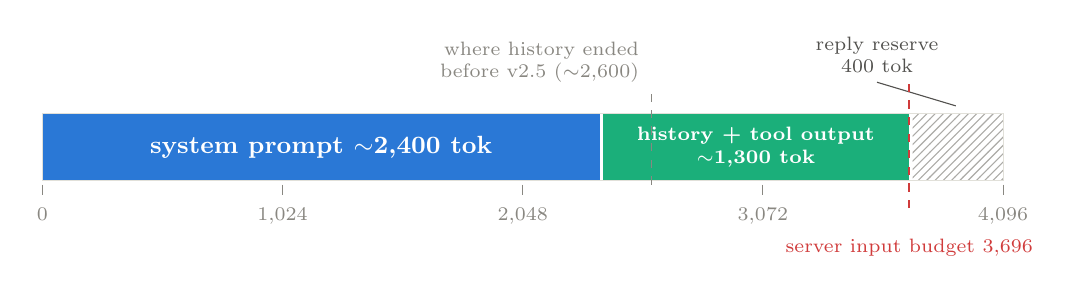
\begin{tikzpicture}[x=1cm, font=\small]
% 4,096 tokens on 12.2cm; prompt 2,377 -> 7.08cm; to the 3,696 budget -> 11.01cm; reply reserve 400 -> 12.2cm
\fill[hexblue]  (0,0)    rectangle (7.08,0.85);
\fill[hexaqua]  (7.12,0) rectangle (11.01,0.85);
\fill[pattern=north east lines, pattern color=hexgray!70] (11.05,0) rectangle (12.2,0.85);
\draw[rulegray] (0,0) rectangle (12.2,0.85);
\node[white, font=\small\bfseries] at (3.54,0.425) {system prompt $\sim$2{,}400 tok};
\node[white, font=\scriptsize\bfseries, align=center] at (9.06,0.425) {history + tool output\\$\sim$1{,}300 tok};
\node[font=\scriptsize, color=inkmuted, align=center] (rsv) at (10.6,1.6) {reply reserve\\400 tok};
\draw[color=inkmuted, thin] (rsv.south) -- (11.6,0.95);
\draw[hexred, thick, dashed] (11.01,-0.35) -- (11.01,1.3);
\node[font=\scriptsize, color=hexred, anchor=north] at (11.01,-0.62) {server input budget 3{,}696};
\draw[hexgray, thin, dashed] (7.74,-0.05) -- (7.74,1.1);
\node[font=\scriptsize, color=hexgray, anchor=south east, align=right] at (7.7,1.12) {where history ended\\before v2.5 ($\sim$2{,}600)};
\foreach \x/\lab in {0/0, 3.05/{1{,}024}, 6.1/{2{,}048}, 9.15/{3{,}072}, 12.2/{4{,}096}} {
  \draw[color=hexgray] (\x,-0.05) -- (\x,-0.18);
  \node[font=\scriptsize, color=hexgray, anchor=north] at (\x,-0.22) {\lab};
}
\end{tikzpicture}
\caption{The 4{,}096-token window as the agent budgets it at v2.8.0. The
server derives a 3{,}696-token input budget from the compiled bundle; the
harness sizes history (about 810 tokens after a 500-token turn reserve) and
tool-output pages against what the prompt leaves. Until v2.5 a
``degradation cliff'', later traced to a parser bug, and a 3{,}000-token
server cap ended history at the grey line.}
\label{fig:window}
\end{figure}

Local inference is a solved problem: Ollama and llama.cpp run this model in
one command, and agents such as aider, Claude Code and Copilot CLI define
what a coding agent should do. What neither side provides is an agent that
stays competent and safe when the model behind it is an order of magnitude
smaller than the one the agent was designed around and the window is a
tenth the size. That gap, on hardware that laptops now ship with, is what
this report is about, and its thesis is that at this scale the harness
(parsing, context management, edit application, safety) matters more than
the model.

% ═══════════════════════════════════════════════════════════════
\section{System}

The system is two layers in two languages (Figure~\ref{fig:arch}). A Python
harness owns the agent loop: prompt construction, action parsing, dispatch
across 15 tools, safety checks, context compaction and the REPL. A fork of
\emph{npurun}, written in Rust, owns inference: it wraps Qualcomm's Genie SDK
behind a local server that speaks the OpenAI API. The fork is not a passive
dependency: it gained exact token accounting, stop sequences, a crash fix,
and later the KV-cache rewind, a bundle-derived budget and a request
watchdog (\S\ref{sec:runtime}). Inference occupies the NPU while the harness
and every tool it runs execute on the CPU cores, so tools never compete with
token generation.

\begin{figure}[ht]
\centering
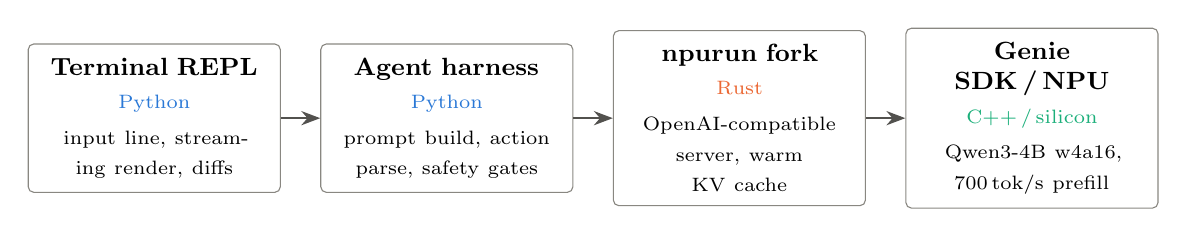
\begin{tikzpicture}[
  node distance=5mm,
  box/.style={draw=hexgray, rounded corners=2pt, align=center,
              inner sep=5pt, minimum height=1.7cm, text width=2.85cm, font=\small},
  arr/.style={-{Stealth[length=2.4mm]}, thick, color=inkmuted}
]
\node[box] (repl)    {\textbf{Terminal REPL}\\[1pt] {\color{hexblue}\scriptsize Python}\\[2pt] \scriptsize input line, streaming render, diffs};
\node[box, right=of repl] (harness) {\textbf{Agent harness}\\[1pt] {\color{hexblue}\scriptsize Python}\\[2pt] \scriptsize prompt build, action parse, safety gates};
\node[box, right=of harness] (npurun) {\textbf{npurun fork}\\[1pt] {\color{hexorange}\scriptsize Rust}\\[2pt] \scriptsize OpenAI-compatible server, warm KV cache};
\node[box, right=of npurun] (npu)    {\textbf{Genie SDK\,/\,NPU}\\[1pt] {\color{hexaqua}\scriptsize C++\,/\,silicon}\\[2pt] \scriptsize Qwen3-4B w4a16, 700\,tok/s prefill};
\draw[arr] (repl) -- (harness);
\draw[arr] (harness) -- (npurun);
\draw[arr] (npurun) -- (npu);
\end{tikzpicture}
\caption{One agent turn. The evaluation instrument drives the same harness
code path the user does: one loop, no test double. The model is quantized to
w4a16 to fit the NPU. Python's share of a turn is below 1\% of wall-clock,
which is why a Rust rewrite was considered and declined.}
\label{fig:arch}
\end{figure}

A session is a conversation in the terminal; each step is a tool call or a
final answer. A representative task from the evaluation suite:

\begin{center}
\fbox{\parbox{0.92\textwidth}{\small
\ttfamily\textcolor{hexblue}{>}\ fix the crash in report.py\\[4pt]
\begin{tabular}{@{}p{2.2cm}p{2.4cm}l@{}}
\ttfamily read\_file  & \ttfamily report.py & \small locates the function \\
\ttfamily run\_code   & \ttfamily report.py & \small NameError: name `conut' is not defined \\
\ttfamily edit\_file  & \ttfamily report.py & \small\ttfamily conut = 0 \rmfamily$\;\rightarrow\;$\ttfamily count = 0 \\
\ttfamily run\_code   & \ttfamily report.py & \small exit 0, output correct \\
\end{tabular}\\[4pt]
\rmfamily\small Fixed. Line 12 of \code{report.py} misspelled \code{count};
corrected and re-run to confirm.}}
\end{center}

Every file mutation is shown as a diff, and a claim of ``done'' after an
unverified edit is deflected: the harness asks the agent to check its work
before it may finish.

% ═══════════════════════════════════════════════════════════════
\section{Method: build the instrument first}
\label{sec:method}

The rule for v2 was that no change ships on intuition. Before touching the
agent, the project built an evaluation instrument with three properties
informal evaluations lack. Grading is based on state: a task passes only if
the filesystem ends up correct or the answer is verifiably right, because a
transcript containing an expected string proves nothing. Every case runs
three to five times and passes only if all runs pass
(pass\textsuperscript{k}), with Wilson intervals; three apparent regressions
in this project vanished when re-run at $n{=}5$ or $10$. And backend failures
are quarantined: the NPU stack silently degrades after an hour or two of
traffic and then looks exactly like a model regression, so the runner marks
runs on a degraded server invalid rather than failed, and every A/B starts a
fresh server per arm. Twice, an apparent regression was the platform
drifting between runs.

% ═══════════════════════════════════════════════════════════════
\section{Results}

Three measurement campaigns produced the numbers here: the v2.0 harness
rebuild in July, the context and runtime work of August and September
(\S\ref{sec:runtime}), and a backend study in September.

\subsection{Same model, rebuilt harness}

The v2.0 gains came from finding the harness's real failure classes. The
largest single fix was in the action parser: a greedy JSON-extraction regex
was silently discarding the model's batched multi-action responses, which
was the true cause of a multi-turn collapse that had been blamed on context
length. A four-tier fuzzy matcher now applies edits (the most common v1
failure was edit formatting, not model capability), malformed actions are
retried with feedback naming the defect, and compaction was recalibrated
with an exact token estimator. Figure~\ref{fig:evals} shows the effect.

\begin{figure}[ht]
\centering
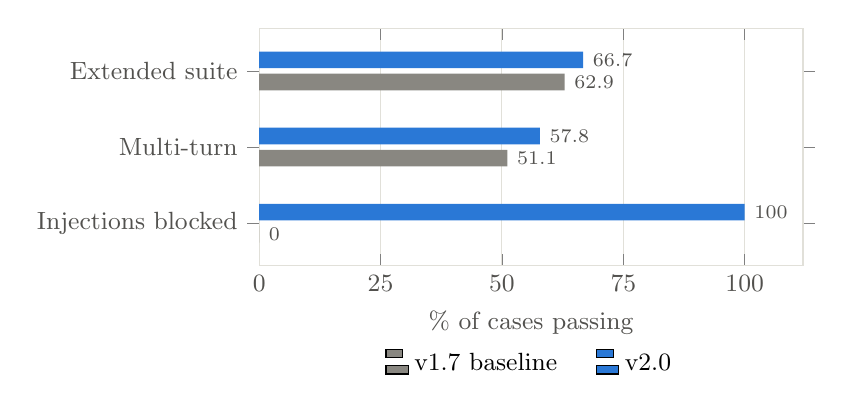
\begin{tikzpicture}
\begin{axis}[
  xbar, xmin=0, xmax=112,
  width=0.7\textwidth, height=4.6cm,
  symbolic y coords={Injections blocked, Multi-turn, Extended suite},
  ytick=data, yticklabel style={font=\small},
  bar width=6pt,
  enlarge y limits=0.28,
  xlabel={\small \% of cases passing}, xlabel style={color=inkmuted},
  xtick={0,25,50,75,100},
  nodes near coords, nodes near coords align={horizontal},
  every node near coord/.append style={font=\scriptsize, color=inkmuted,
    /pgf/number format/fixed, /pgf/number format/precision=1},
  legend style={at={(0.5,-0.32)}, anchor=north, legend columns=-1,
                draw=none, font=\small, /tikz/every even column/.append style={column sep=12pt}},
  axis line style={color=rulegray},
  xmajorgrids, grid style={color=rulegray},
  tick label style={font=\small, color=inkmuted},
]
\addplot[fill=hexgray, draw=none] coordinates
  {(62.9,Extended suite) (51.1,Multi-turn) (0,Injections blocked)};
\addplot[fill=hexblue, draw=none] coordinates
  {(66.7,Extended suite) (57.8,Multi-turn) (100,Injections blocked)};
\legend{v1.7 baseline, v2.0}
\end{axis}
\end{tikzpicture}
\caption{v1.7 and v2.0 on identical model and hardware. Extended suite:
22/35 to 24/36 cases passing all five runs (the suite gained a case).
Multi-turn: 23/45 to 26/45 turn-runs. Injection payloads blocked: 0/9 to
9/9.}
\label{fig:evals}
\end{figure}

\subsection{Where the window goes}

Budgeting the prompt produced the most counter-intuitive finding of the
project. Of the 1{,}990-token template at v2.0, the 14 behavioural rules were
73\% and all 15 tool schemas about 450 tokens, so consolidating tools would
have saved almost nothing, and \S\ref{sec:negative} shows the rules could not
be trimmed either. By v2.2 a live-state cookbook (which lifted machine-state
questions from 44\% to 72\%) had grown the prompt to 2{,}355 tokens, measured
from the server's usage report, and auto-compaction fired every few messages.
Compaction itself was the thrash: the compactor re-fired every turn and
crushed its own summary into a stub. Making it merge-aware with a dry-run
gain guard fixed the churn without touching the prompt. The history floor
that remained was taken for a property of the model; \S\ref{sec:runtime}
records that it was not.

\subsection{Why the NPU, when the CPU decodes faster}

On plain CPU the same model decodes faster than the NPU path (13.5 versus
8.1 tokens per second in the v2.0 test), but an agent re-reads its prompt,
and prefill is where the NPU is untouchable: 4.1\,s to first token against
13.6\,s on CPU for the same 2{,}100-token prompt, arms interleaved. Extending
the two measured points across turn lengths (Figure~\ref{fig:crossover}), the
CPU would pay off only past about 193 generated tokens per turn, and real
turns generate 12 to 126. A second study in September under the warm-cache
runtime (\code{docs/backend\_study/CPU\_VS\_NPU.md}) kept the conclusion and
sharpened the numbers: the NPU decodes at 15.5 tokens per second at short
context and 9--10 at the agent's working context; a cold prefill of 2{,}048
tokens takes 8.3\,s; a warm follow-up turn reaches its first token in about
0.8\,s, and a new conversation pays a 6.6--8\,s dialog rebuild only when the
system prompt changes, which the byte-stable prefix avoids (an earlier
``9\,s per new conversation'' was the benchmark's own nonce forcing the
rebuild, and is retracted). Switching off the runtime's host-side polling
raised decode to 19 tokens per second while cutting package power from
21\,W to 9.8\,W, 0.55\,J per token instead of 1.44, with no quality change
(62/82 against 61/82).

\begin{figure}[ht]
\centering
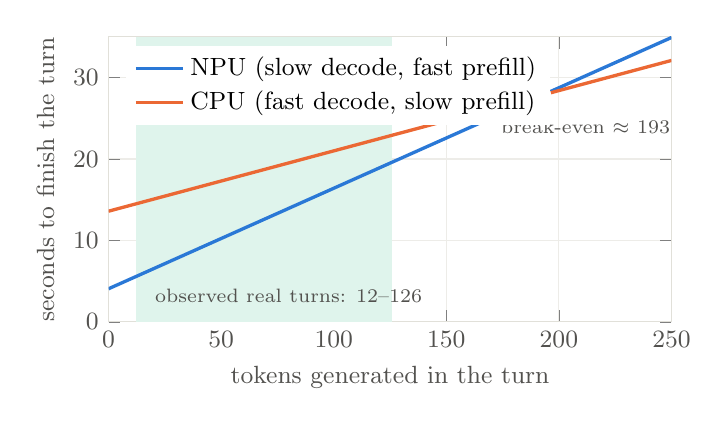
\begin{tikzpicture}
\begin{axis}[
  width=0.72\textwidth, height=5.2cm,
  xmin=0, xmax=250, ymin=0, ymax=35,
  xlabel={\small tokens generated in the turn}, xlabel style={color=inkmuted},
  ylabel={\small seconds to finish the turn}, ylabel style={color=inkmuted},
  axis line style={color=rulegray},
  grid, grid style={color=rulegray!60},
  tick label style={font=\small, color=inkmuted},
  legend style={draw=none, font=\small, at={(0.03,0.97)}, anchor=north west},
  legend cell align=left,
]
\fill[hexaqua!14] (axis cs:12,0) rectangle (axis cs:126,35);
\node[font=\scriptsize, color=inkmuted, align=center, anchor=south] at (axis cs:80,1.2)
  {observed real turns: 12--126};
\addplot[hexblue, very thick, domain=0:250, samples=2] {4.06 + x/8.1};
\addlegendentry{NPU (slow decode, fast prefill)}
\addplot[hexorange, very thick, domain=0:250, samples=2] {13.59 + x/13.5};
\addlegendentry{CPU (fast decode, slow prefill)}
\addplot[forget plot, only marks, mark=*, mark size=2.4,
  mark options={fill=hexred, draw=white, line width=1pt}] coordinates {(193,27.9)};
\node[font=\scriptsize, color=inkmuted, anchor=north west] at (axis cs:170,26)
  {break-even $\approx$ 193 tok};
\end{axis}
\end{tikzpicture}
\caption{Turn time against tokens generated, from the v2.0 intercepts and
decode rates (NPU: 4.06\,s + 8.1 tok/s; CPU llama.cpp Q4\_0: 13.59\,s +
13.5 tok/s). The CPU wins only right of the break-even, and real turns never
get there.}
\label{fig:crossover}
\end{figure}

\subsection{What still fails}

Section 1 asked how much of a coding agent survives at this scale, and the
honest answer includes the failures: 12 of 36 cases at v2.0, and 12 of 44 at
v2.8.0, seven of them at 0 of 5 runs. They fall in two classes, both model
ceilings. Bait compliance: when a prompt names a tool (``use
\code{run\_command} to\ldots'') for something that should be answered
directly, the model complies about one time in three despite a rule against
it; three of the seven hard failures are these. Edit anchoring: on a
follow-up turn the model reconstructs an \code{edit\_file} anchor from memory
instead of from the file, three times in a row, or describes the change in
prose instead of making it. The harness turns both from silent failures into
retried or deflected ones; it cannot eliminate them. They mark where a better
small model would help, and the instrument can judge one in an afternoon.

% ═══════════════════════════════════════════════════════════════
\section{The runtime lever}
\label{sec:runtime}

The largest gain after v2.0 came from the runtime, not the prompt. A
2{,}355-token system prompt prefilled again on every agent step is a fixed
tax of about five seconds per call, and the Genie runtime in QAIRT~2.47
rejects its own KV-cache rewind on this bundle. QAIRT~2.50 accepts it. The
fork now keeps one dialog alive for the life of the process and sends every
warm query as a prefix-matching rewind, rebuilding the dialog only when the
system prompt changes; two runtime behaviours dictated that shape (a reset
after a large prefill wedges the dialog, and an early-diverging transcript
poisons it). The prompt had to become byte-identical across directories and
days, which moved the date and working directory into the first user
message. Measured on the extended suite, three runs per case, fresh server
per arm: run-level 91/117 $\to$ 97/117 (Fisher $p=0.41$), first-token median
6.8\,s $\to$ 3.7\,s, later steps 7.6\,s $\to$ 3.2\,s, whole-turn mean 16.0\,s
$\to$ 9.5\,s.

With the prefill tax gone, the context question could be re-read. The
250-token history floor rested on two constants nobody had derived: the
harness's 2{,}600-token ``degradation cliff'' (the collapse it described was,
by the project's own record, the parser bug of \S4.1) and a 3{,}000-token
input cap inherited from upstream. The bundle is compiled to 4{,}096. A sweep
at controlled input sizes found quality flat from 2{,}370 to 3{,}697 tokens,
the same three cases failing at every size, and decode about 12\% slower
only with the window actually full. The server now derives its budget from
the bundle (3{,}696 after a reply reserve) and advertises it; the harness
sizes history and tool pages against it, lifting history to about 800
tokens. Two defects surfaced only in multi-turn measurement: a rewind on a
transcript that diverges mid-conversation can return success with zero
tokens (63 of 117 calls in one run; now treated as a failed rewind), and a
divergent rewind fails outright past roughly 3{,}200 cached tokens, which an
end-of-turn prewarm absorbs in the background. Multi-turn went from 25/48 to
35/48 turn-runs and server trims per run from 141 to 17, with the extended
suite at parity.

% ═══════════════════════════════════════════════════════════════
\section{Negative results}
\label{sec:negative}

Half the value of the instrument is what it stopped from shipping
(Table~\ref{tab:rejected}). One finding runs under several rows: a small
model tuned for months against one prompt becomes specialized to that exact
prompt. Dropping even provably irrelevant rules degraded behaviour, and
removing one rule hurt more than removing four. At this scale the prompt is
not documentation the model consults; it is part of the distribution the
model has adapted to, and that holds at every step of the loop, not just the
first. The one split that survived was the one that changes the model's task
rather than shrinking its prompt: a harness-routed no-tools stage for
pure-knowledge queries, which cut their first-token latency by 40\%
(10.1\,s $\to$ 6.0\,s median). It is switched off under the warm-cache
runtime, where a knowledge query is already decode-bound and a second system
prompt would only buy a rebuild.

\begin{table}[ht]
\centering\small
\begin{tabular}{@{}p{4.2cm}p{8.0cm}l@{}}
\toprule
\textbf{Idea} & \textbf{What the measurement said} & \textbf{Verdict} \\
\midrule
New structured \code{<action>} protocol &
13/36 vs.\ 22/35 pass\textsuperscript{5}; two months of tuning had
specialized the model to the old format & rejected \\[2pt]
Prompt trimming (drop situationally irrelevant rules) &
saved 690 tokens and 16\% latency, but bait resistance fell from 5/8 to 3/18
($p \approx 0.017$), and the damage did not scale with rules dropped & rejected \\[2pt]
8K context window (recompiled bundle) &
6 tok/s vs.\ 15, no quality gain & rejected \\[2pt]
Raise the compaction threshold &
flat from 2{,}370 to 2{,}973 tokens but capped at $\sim$3K, so closed as
``zero usable history''; the cap was a server constant, a second sweep was
flat to 3{,}697, and history went 250 $\to$ $\sim$800 (\S\ref{sec:runtime}) & reversed \\[2pt]
Leaner prompt for steps $\ge 2$ &
quality flat (77.8\% vs.\ 74.4\%, $p=0.65$), but the JSON-edit case fell
3/3 $\to$ 1/3 with degenerate anchors, the trimming fingerprint again & rejected \\[2pt]
Escalate hard cases to Qwen3-8B &
0.9 tok/s: silent CPU fallback on 16\,GB & rejected \\[2pt]
Qwen3.5-4B successor &
20--25\% slower than the incumbent on both CPU and hybrid paths & deferred \\[2pt]
Native Qwen3 \code{<tool\_call>} template &
the quantized bundle's detokenizer garbles its own special token & impossible \\[2pt]
GenieX runtime ($+47\%$ claimed) &
0.74 tok/s here: a fixed 1.5\,s penalty per NPU graph call; filed upstream
(\#1266, PR \#1267) & halted \\[2pt]
Rewrite the harness in Rust &
Python is below 1\% of a turn; the bottleneck is inference & declined \\
\bottomrule
\end{tabular}
\caption{Ten plausible improvements that failed their evaluations, recorded
so none is re-argued from intuition.}
\label{tab:rejected}
\end{table}

% ═══════════════════════════════════════════════════════════════
\section{Security: assume the model is fully injectable}

To a 4B model, a malicious instruction hidden in a README it was asked to
read is indistinguishable from the user. v1.7 executed all nine payloads in
the live injection suite (hosts-file reconnaissance, SSH-key exfiltration,
spawning executables); v2.0 blocks all nine, and the principle matters more
than the score: no defense may depend on the model resisting the bait.
Enforcement lives in the harness. A \emph{sensitive} tier above ``safe''
covers credential stores, SSH and cloud keys, registry hives and
encoded-command tricks, confirmed interactively and denied when unattended;
every mutating path routes through one \code{guard\_mutation} gate, and a
test enumerates every mutating entry point against a forbidden path; the one
tool that reaches the network asks before every fetch. One measured lesson
became a style rule: an early refusal message suggested an alternative
command and the model followed it straight to the bypass, so refusals never
name another route. Packaging in v2.8.0 found the classifier's own blind
spot: it had treated every \code{Format-} verb as a disk format, so the
\code{Format-List} the model appends to live-state queries asked for a
confirmation that unattended evals answer with a denial. The live-state
numbers above carry that handicap; the fix is a two-line pattern.

% ═══════════════════════════════════════════════════════════════
\section{Lessons}

\begin{enumerate}[itemsep=2pt]
\item \textbf{At small scale, the harness is the product.} Every measured win
(parsing, edit application, compaction timing, retry feedback, the warm
cache) came from the scaffolding around a frozen model.
\item \textbf{Build the instrument before the feature.}
pass\textsuperscript{k} with state-based grading made every claim here
possible and repeatedly overturned the story a single run told.
\item \textbf{Interrogate the measurement platform.} A silently degrading
backend impersonates a model regression perfectly.
\item \textbf{Security is a property of the architecture, not the model.}
Assume total injectability; put every enforcement decision in code you
control; test it by enumeration.
\item \textbf{Negative results are deliverables.} Written down with their
evidence, they keep future work from re-fighting settled questions.
\item \textbf{Mechanics beat prose.} Twice in v2.7 a prompt sentence fixed
one case and broke a gated one; a loop nudge (``run the tests'' means a test
ran, 0/5 $\to$ 5/5) and a loop guard (no edit lands on a file the request did
not name, 1/5 $\to$ 5/5) did the job without touching the prompt.
\end{enumerate}

% ═══════════════════════════════════════════════════════════════
\section{Status}

At v2.8.0 the agent runs in Windows Terminal with a pinned input box and
status line, prints only the answer when its output is a pipe, and installs
from PyPI (\code{pip install hexcli}). The headline is 32 of 44 cases at
pass\textsuperscript{5} on a fresh server and 35 of 48 multi-turn turn-runs;
the multi-turn suite still loses about one run in three near 3{,}100 tokens
to a platform stall that the server's watchdog now ends in 97\,s rather than
400, counted as a backend failure. What remains on the harness side is small:
compaction sharing the warm prefix, paging of large files, and the
edit-anchoring case. The other levers need a different model or runtime,
and when a successor bundle appears for this NPU the instrument can judge it
in an afternoon.\footnote{All figures were measured on a Snapdragon X~Elite
(X1E78100), 16\,GB RAM, Windows 11 ARM, with Qwen3-4B-Instruct-2507 (w4a16)
on the Hexagon NPU. Method and run-level data: \code{docs/V2\_PLAN.md} \S14,
\code{docs/backend\_study/} and \code{evals/results/} in the repository.}

{\small
\begin{longtable}{@{}lp{12.4cm}@{}}
\caption{Milestones, 2026.}\label{tab:timeline}\\
\toprule
\textbf{Date} & \textbf{Milestone} \\
\midrule
\endfirsthead
\toprule
\textbf{Date} & \textbf{Milestone} \\
\midrule
\endhead
\bottomrule
\endlastfoot
Jun 16 & First end-to-end NPU inference at about 15 tok/s, after two other runtimes proved dead ends. \\
Jul 30--31 & v2.0: instrument v2, loop rebuild, injection defense 0/9 $\to$ 9/9, product shell; 619 tests. \\
Aug 14 & v2.1: one-command installer, piped stdin, custom commands; a review found ten defects, all fixed. \\
Aug 16 & v2.2: live-state cookbook 44\% $\to$ 72\%; the memory daemon found re-injecting the model's own confabulations. \\
Aug 29--31 & Compaction thrash fixed; command surface pruned to one mode ($-685$ lines); prompt-split A/B. \\
Sep 1--2 & Main module split into seven stages (3{,}818 $\to$ 1{,}499 lines); KV rewind on QAIRT 2.50, $-41\%$ turn time; context floor traced to two constants and lifted. \\
Sep 5--7 & CPU-versus-NPU study; host-polling control, async init and the request watchdog (v2.6.x). \\
Sep 10--12 & Windows Terminal surface; loop nudge and named-file guard through the gate; v2.7--2.8; PyPI package; Format-List classifier fix. \\
\end{longtable}}

\end{document}
